%-------------------------------------------------------------------------------
\section{Introduction}
%-------------------------------------------------------------------------------

% \thea{I think the motivation could be more focused. As I'm understanding it,
%  I think the core motivation/background should be: Connection-splitting PEPs
%  improve end-to-end throughput (1) on high-loss and/or high-latency network
%  paths when (2) end-hosts are running loss-based CCAs -- this isn't really
%  controversial. There's debate: --> with the development of delay-based CCAs
%  (BBR) and QUIC, debate about how big these improvements actually are in
%  practice (and whether they are worth the risk of ossification)
% *For this, cite Google's claims about QUIC, fact that BBR uses delay, and
%  something that's pro-PEP [maybe from satellite networks research?]* Where we
%  come in: points for a need for tools that support reasoning about PEPs in
%  modern networks}

\begin{figure}[t!]
    \centering
    \begin{subfigure}[b]{0.49\linewidth}
        \centering
        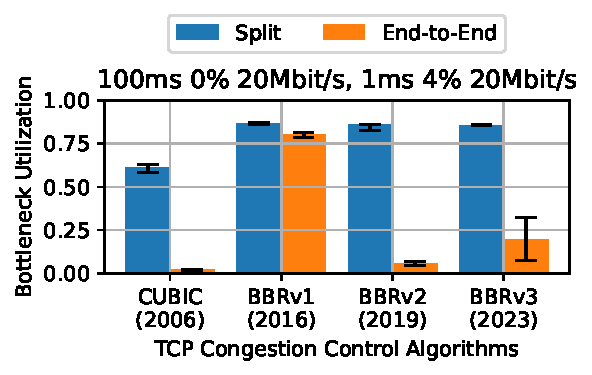
\includegraphics[width=\linewidth]
         {splitting/figures/bbr_over_time_network_20_20_100_1_None_None_0_4.pdf}
        \captionsetup{skip=0pt}
        \caption{Asymmetric, lossy last-mile.}
        \label{fig:splitting:bbr-over-time:class1}
    \end{subfigure}
    \begin{subfigure}[b]{0.49\linewidth}
        \centering
        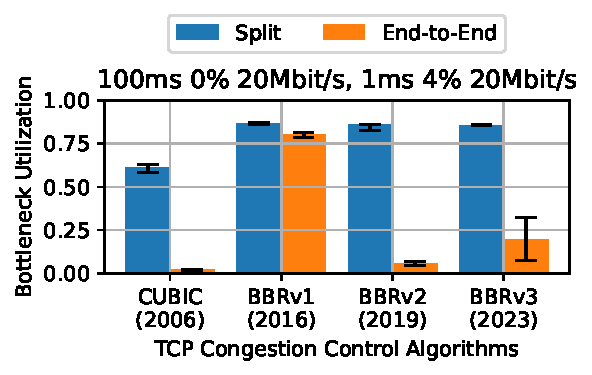
\includegraphics[width=\linewidth, trim=0 155 0 0]
         {splitting/figures/bbr_over_time_network_20_20_100_1_None_None_0_4.pdf}
        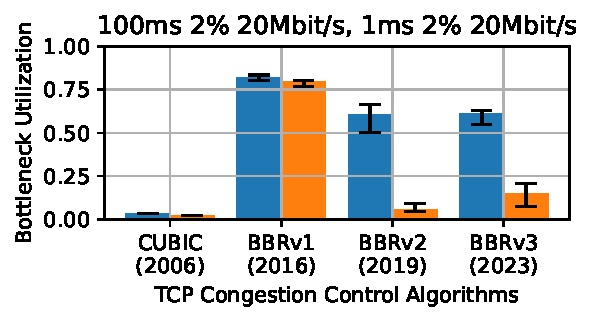
\includegraphics[width=\linewidth]
         {splitting/figures/bbr_over_time_network_20_20_100_1_None_None_2_2.pdf}
        \captionsetup{skip=0pt}
        \caption{Asymmetric, both path segments are lossy.}
        \label{fig:splitting:bbr-over-time:class2}
    \end{subfigure}
    \begin{subfigure}[b]{0.49\linewidth}
        \centering
        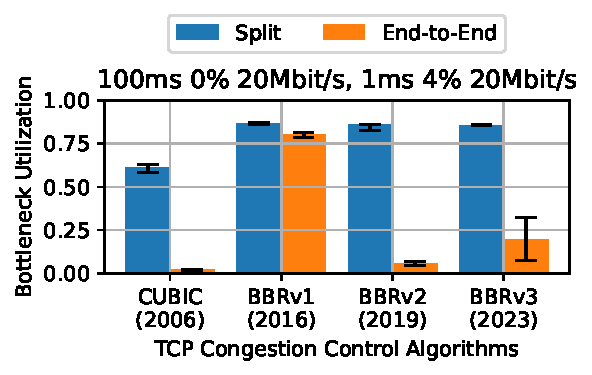
\includegraphics[width=\linewidth, trim=0 155 0 0]
         {splitting/figures/bbr_over_time_network_20_20_100_1_None_None_0_4.pdf}
        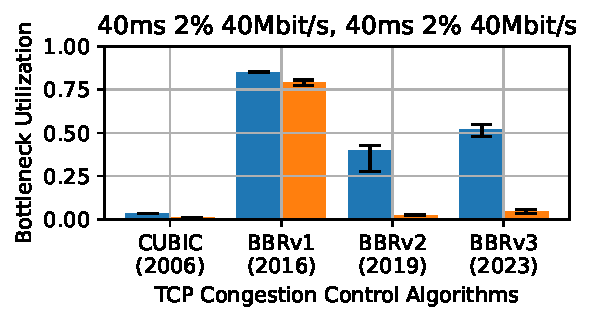
\includegraphics[width=\linewidth]
         {splitting/figures/bbr_over_time_network_40_40_40_40_None_None_2_2.pdf}
        \captionsetup{skip=0pt}
        \caption{Symmetric, both path segments are lossy.}
        \label{fig:splitting:bbr-over-time:class3}
    \end{subfigure}
    \caption{Three classes of network settings in which the throughput of a
     long-lived data transfer using BBRv3 benefits significantly from
     connection-splitting. While the throughput of TCP using BBRv1 may not have
     benefitted from a PEP, as the BBR algorithm has evolved over time, it has
     also made connection-splitting pertinent again. In two of these classes,
     split BBRv3 even achieves high bottleneck link rate utilization where split
     CUBIC does not. IQR of $n=20$.}
    \label{fig:splitting:bbr-over-time}
\end{figure}


A stylized history of connection-splitting over the Internet could go
roughly as follows: In the 1970s, TCP was designed as a host-to-host
transport for flow-controlled reliable byte streams. In the late
1980s, TCP implementations added congestion control~\cite{vjk} to
respond to network-path limitations and contention, with indications
of packet loss as the primary congestion signals. As Internet use
exploded in the 1990s, it became apparent that contemporary TCP
implementations performed poorly over long paths with packet loss. By
the late 1990s, many network operators deployed commercial ``TCP
accelerators,'' also known as ``performance-enhancing proxies''
\cite{rfc3135, honda2011still}, to improve customers' TCP
throughput. These proxies transparently split a TCP connection in two,
providing an intermediate point of acknowledgment and retransmission
and transforming an end-to-end TCP connection into two independent
connections.

PEPs were marketed as improving users' throughput, especially where a
PEP splits a high-delay, lossy path into two segments, each with less
delay or less loss. Past surveys found connection-splitting PEPs
deployed on large numbers of wireless and satellite
networks~\cite{rfc3135, honda2011still}. But for almost as long as
these PEPs have existed, purists have criticized their alleged
benefits as exaggerated or unfair, sensitive to the details of an
endpoint's congestion-control scheme, contrary to end-to-end
arguments~\cite{Saltzer84}, and likely to lead to
ossificiation~\cite{papastergiou2017deossifying, edeline2019bottomup}.

Two more-recent developments have put PEPs on the back foot. The QUIC
transport protocol, standardized in 2021~\cite{rfc9000}, is encrypted
end-to-end and, unlike TCP, its connections can't be split by a
transparent proxy---but its wide deployment by major traffic sources (particularly Google)
in the 2010s didn't produce a measured reduction in performance,
compared with TCP connections that do benefit from PEPs in the
field~\cite{langley2017quic}. If PEPs had really been aiding TCP connections all this time,
QUIC could have been expected to experience lower sustained throughput
over such paths (compared with TCP connections between the same
endpoints, using the same congestion-control schemes).

Furthermore, the BBR congestion-control scheme~\cite{cardwell2017bbr}, first
released in 2016, now controls a large percentage of Internet traffic
(both TCP and QUIC)~\cite{ware2024ccanalyzer} and puts less emphasis on packet
loss as a congestion signal than older schemes in wide
deployment, such as CUBIC. Because much of PEPs' benefit comes from
splitting up long, lossy paths for the benefit of ``loss-based''
schemes, it has been suggested that BBR has led to
a sharp decline in the use of PEPs~\cite{frode}.

\textbf{Do BBR and QUIC make connection-splitting obsolete?} In this
paper, we present findings that suggest that neither of these
developments should be regarded as reliable;
Connection-splitting may yet play a performance-enhancing role
on the Internet, despite its controversial nature.

%The experience paper on QUIC also reports on performance, particularly latency,
%improvements across the board~\cite{langley2017quic}, but other measurement
%studies have suggested that QUIC could still stand to benefit from in-network
%assistance~\cite
%{kosek2022quicpep,thomas2019google,deutschmann2023cubic,yuan2024sidekick}.
%\textbf{Do BBR and QUIC make connection-splitting obsolete?}
% Don't necessarily want to cite the Zulip IETF thing here b/c it's just one
% message... not sure what else to cite here?

% \thea{I think this goes into a different section -- too much in the weeds}
%  Meanwhile, new congestion-control schemes have arisen (especially BBR) that do
%  not depend on loss as their primary congestion signal. The idea is that they
%  are resilient to the low link rate utilization on these high-loss networks
%  that previous CCAs had so much trouble with and required PEPs. Certainly, when
%  BBR first came out in 2016, there were measurement studies that said it did
%  not need local loss recovery unlike CUBIC~\cite{}. But as BBR came under hot
%  fire for its aggressiveness and unfairness, the algorithm has evolved since
%  then as BBRv2 and now BBRv3, and its interactions with connection-splitting
%  PEPs are not well studied.

% The current prevailing view may be that connection splitting's time has simply
% passed, but we think there is reason to challenge this. \thea{Is this something
% we can back up?}

We conduct a measurement study in emulation to investigate what kinds of
congestion control schemes, network scenarios, and transport protocols may
still experience increased sustained throughput from connection-splitting. We
aid our analysis with a \textit{split throughput heuristic} for predicting the
throughput of a split
connection, based on the measured end-to-end throughput of each segment on the
split path. We aim to (1) explore a wide parameter space of network settings
and congestion control schemes and (2) reason about encrypted transport
protocols (QUIC) that we cannot directly measure.

% \thea{Proposing to remove this paragraph or move to different section to make
%  intro more concise} \gina{Emulations take time to run; an exhaustive search
%  over a parameter space that includes combinations of path segments is
%  infeasible. Previous studies have often focused on just a handful of network
%  scenarios~\cite{}, often those that reflect existing PEP deployments,
%  typically at the edge~\cite{}. We need to think proactively to reason about
%  opportunities for connection-splitting (e.g., LEO satellite networks).
%  Additionally, we cannot directly measure split QUIC performance with a basic
%  PEP. Previous studies have implemented custom connection splitters for
%  specific implementations~\cite{} or only compared to split TCP~\cite{}, but
%  each QUIC implementation is unique and the results may not generalize.}

%To accomplish this, we make the important insight that we can understand the
%split behavior of a connection (not well-understood) from its end-to-end
%behavior (well-understood). In a simplified network model based on propagation
%delay, bandwidth, and a random loss rate, we define the following
%\textit{split performance heuristic} for the sustained goodput of a single flow:
% We can use the minimum achievable \textit{end-to-end performance} on each path
% segment of a split connection as a heuristic for the maximum \textit
% {split performance} on the network path. This methodology allows us to
% efficiently analyze split performance across a wide variety of scenarios and
% to explore theoretical scenarios where splitting may be beneficial.

% While a similar idea has been proposed \cite{}, prior work does not describe or
% implement a formal heuristic. <-- do we need to include this? can we put it in
% a later section?

% \thea{Need to be clearer about the limitations than is currently in the
%  introduction.} \gina{Incorporate limitations described in \Cref
%  {sec:limitations}?} We implement the heuristic with a network model of delay,
%  link rate, and a random loss rate, and perform the goodput measurement in a
%  mininet emulation.
% \thea{The “3 parameters” aren’t an implementation, they’re core to the
%  heuristic, so would be careful with language here.} This methodology allows us
%  to more efficiently understand split performance for a variety of CCAs and
%  implementations, as well as explore theoretical scenarios where splitting may
%  be beneficial.

%Equipped with this heuristic, what we find in our emulation measurement study is
%basically: It's complicated, but "no," connection-splitting proxies are not
%pointless. While it's true that ISPs may not have benefitted their customers
%using BBRv1, \textit{split connections significantly outperform end-to-end
%connections on a variety of network paths with high loss when using BBRv3.}
We present three major findings:

\paragraph{Finding 1: Splitting has become significantly more beneficial to TCP
 BBR since it was initially released in 2016.}

We confirm that BBR's initial ``v1'' release does not benefit markedly from splitting, unlike earlier
congestion-control schemes. But as the BBR algorithm
has evolved into BBRv2 in 2019 and now BBRv3 in 2023, it has also evolved to
behave more conventionally in the sense that it benefits from being
split---just like more traditional, loss-based congestion control schemes such
as CUBIC (\Cref{fig:bbr-over-time}).

The regression in split throughput follows directly from the regression
in end-to-end throughput, via the heuristic. While BBRv1 nearly always achieves
full utilization, BBRv3 sees lower utilization in lossy
settings, leaving more to gain from splitting.
The end-to-end regression is because BBRv3 has increased its loss sensitivity
to coexist fairly with ``loss-based'' schemes such as Reno and
CUBIC~\cite{cardwell2024bbrv3-ietf119,ware2019modeling,zeynali2024promises}.
% response to loss as a congestion signal -- in part to coexist fairly with
% ``loss-driven'' congestion-control schemes such as Reno and CUBIC~\cite{cardwell2024bbrv3-ietf119},
% and in part to respond to traffic policers that limit end-to-end flows by
% dropping packets if they exceed a given rate. (See also \cite{ware2019modeling,zeynali2024promises}.)
% \gina{I don't actually know any citations for these claims about policing?}
% Many of these changes in the conservative
% direction have been in response to concerns about BBRv1 unfairness~\cite
% {ware2019modeling}, and these concerns remain controversial with BBRv3~\cite
% {zeynali2024promises}.
Thus, we find that BBR and its split behavior continue
to evolve, and that the model-based BBR algorithm has \textit{not} made the
performance enhancements of connection-splitting obsolete.
% (And, in terms of latency, it remains true that saving an end-to-end roundtrip
% on a retransmission can be beneficial, no matter what the congestion-control
% scheme is!) \thea{eh idk, BBRv1 results are not that compelling to this point}

\paragraph{Finding 2: There exist classes of network paths where TCP BBR would
 significantly benefit from splitting but TCP CUBIC would not.}

Splitting not only benefits BBRv3 in all the same scenarios as CUBIC (in terms
of long-lived throughput), it also benefits BBRv3 in \textit{new} scenarios. In
particular, there exist classes of network settings where the CCA achieves a
very low bottleneck link rate utilization \textit{without} a PEP, but a high
bottleneck link rate utilization \textit{with} a PEP.

More specifically, in addition to edge deployments with a lossy last-mile (\Cref
{fig:bbr-over-time:class1}), BBRv3 can also benefit from splitting in
scenarios where there is loss on both path segments (\Cref
{fig:bbr-over-time:class2}), and when the connection-splitter is located
farther from the edge (\Cref{fig:bbr-over-time:class3}). This suggests that in
these network classes, simple split BBRv3 can replace the
proprietary protocols that have traditionally been used to address middle-mile
loss, particularly in satellite and wireless ad-hoc networks~\cite
{cloudsplitting2010,border2022evaluating,rfc3135}. We should continue to
evaluate the behavior of split CCAs in new types of networks, especially in
space.

% While TCP CUBIC only benefits from connection-splitting when the PEP is located
% at the lossy last-mile, TCP BBRv3 can also benefit when there is loss on both
% sides of the PEP and when there are longer propagation delays. This suggests
% that TCP connections using BBRv3 should benefit from splitters at the same
% locations as for CUBIC, and also that traditionally invasive methods used to
% address loss in the middle-mile could use simple connection-splitting instead.
% We believe this method of analyzing useful network paths and PEP placements for
% connection-splitting can be extended to model new types of networks, especially
% in space.

% \thea{in later section, connect to analogous real-world scenarios} This is
%  important with the development of space networks where weather conditions and
%  fast-moving orbits have high loss.
% \thea{I like the framing of "why this is important", though I’d use slightly
%  more specific language? Speak to the continued performance contribution of
%  connection-splitting PEPs with (1) the evolution of BBR and (2) the importance
%  of high-loss and high-latency networks (satellite, ad-hoc wireless, maybe
%  cellular?) for expanding Internet access Possible value in investing in PEPs
%  for encrypted transport protocols Support network operators to reason about
%  PEP deployment and placement.}

% Keith: In terms of long-lived, single-stream throughput, we hypothesize that
% QUIC benefits from TCP connection splitting

\paragraph{Finding 3: Implementations of the ``same'' congestion-control schemes
in QUIC vary significantly, and further differ those of Linux TCP---frustrating
attempts to directly compare performance between QUIC and TCP.}

In an initial study of three QUIC implementations, we find that the end-to-end
behaviors of the same congestion control schemes vary significantly by implementation.
The implementations vary in both baseline performance and sensitivity to loss
and delay. By applying the split throughput heuristic, we find that some
CUBIC implementations can actually benefit in the same classes of network paths
as TCP BBRv3. We also find that BBR is challenging to implement, with various
BBRv3 implementations exhibiting non-uniform end-to-end behavior and thus no
clear trend in split behavior. We argue that the benefits of in-network
assistance should be considered along with not just a CCA, but their specific
implementations. \\

% \paragraph{Finding 3: Some QUIC implementations indeed have less, but others
%  have \textit{more} to gain than TCP by connection-splitting.}
% \paragraph{Finding 3: If QUIC's split performance is dominated by congestion
%  control, then QUIC is losing out on long-lived, single-stream throughput by
%  not connection-splitting.} Prior work has demonstrated that, in certain
%  network scenarios, TCP with a connection-splitting PEP outperforms end-to-end
%  QUIC~\cite{} and that QUIC stands to benefit from in-network assistance~\cite
%  {}. We apply our heuristic to estimate the benefits of a simple connection
%  splitter for various CCA implementations of QUIC. We hypothesize that, in some
%  network settings, connection-splitting would increase QUIC throughput, but the
%  particulars depend on the specific implementation (e.g., Cloudflare quic-bbr
%  vs. Google quic-bbr).

% In summary, we make the following contributions:
% \begin{itemize}[noitemsep]
%     \item A heuristic for deriving split performance (not well-understood) from
%      end-to-end performance (well-understood) of a CCA, and an evaluation of
%      its accuracy in emulation.
%     \item A measurement study of the impact of connection-splitting PEPs on a
%      variety of netework settings, CCAs, transport portocols, and their
%      implementations, and three main findings.
% \end{itemize}

\noindent Our initial evaluation suggests that the performance improvements of
connection-splitting remain relevant in the context of today's model-based
congestion control algorithms, encrypted transport protocols, and satellite and
wireless ad-hoc network settings. As congestion-control schemes continue to
evolve, we urge researchers to refer to them by
algorithm/implementation/version, not just ``BBR'' or even ``QUIC BBRv1''. We
urge the community to create a performance test suite for an implementation to
be able to claim that it conforms to a particular congestion-control standard.
Finally, we hope that this work motivates the community to pursue
protocol-agnostic PEPs that achieve the performance benefits of in-network
assistance without the ossification downsides.

% Connection-splitting TCP performance-enhancing proxies split an end-to-end TCP
% connection into multiple segments, each with their own parameters to transfer
% data based on the particulars of each path segment. This alleviates known
% performance issues such as low throughput over high-BDP links and small
% receive-side flow control windows.

% Split TCP PEPs are widely deployed in networks composed of very different path
% segments. Satellite networks have a long backhaul and two shitty ground
% segments. Cellular networks to account for the last mile. Companies are open
% about their deployment of TCP PEPs, but research studies typically focus on
% their negative effects. In fact, it is challenging to characterize their
% performance benefits in the wild. But since they are deployed, what's so good
% about them?

% One is it divides the path segments into lower BDP networks, and congestion
% control algorithms are known to be unable to utilize their fair share in high
% BDP networks. Especially loss-based congestion control algorithms such as CUBIC
% and Reno are sensitive to signals about loss, but are there any benefits to
% BBR? Paradigm is that split congestion control is like an entirely different
% algorithm from the original congestion control algorithm itself.

% The other is that an earlier signal about loss and buffering at the PEP
% necessarily allow for earlier retransmission. This can reduce the tail latency
% of short connections by a noticeable amount. Based on the results of the
% performance analysis in varying network conditions, we make recommendations on
% what types of networks connection-splitting PEPs can be most beneficial.

% Fairness study on how split TCP connections affect concurrent flows. If the
% concurrent connections are split then fairness properties are necessarily the
% same along each path segment. But increasingly transport protocols like QUIC
% are encrypted and cannot benefit from PEPs. How does the congestion control of
% split TCP connections do in fairness alongside an end-to-end congestion control
% like QUIC?

% There are many PEPs in the world that do various things with ACKs. RFC 3135. We
% focus specifically on the connection-splitting TCP PEP. It intercepts the SYN
% in the connection and forms two separate split TCP connections. When it
% receives a packet from one end of the connection, it immediately tries to send
% it on the other side. The buffers are implemented entirely in the Linux kernel
% and are subject to configurations there.

% The most popular congestion control algorithms are CUBIC, the default in the
% Linux kernel, and BBR. BBR is used by many companies and comes in multiple
% versions, most companies deploy v1 but Google is pushing v3 as the standard due
% its improved fairness. BBRv3 is now in the mainline Linux kernel as the default
% BBR module, indicating that the usage of v1 is highly discouraged. In this
% paper, we evaluate CUBIC, BBRv3 (BBR), and BBRv1 for legacy reasons.

% When a congestion control algorithm operates end-to-end, we refer to it by its
% original name, e.g., CUBIC. When speaking about the performance of and
% end-to-end connection using a congestion control algorithm in a split TCP
% connection, we refer to this treatment as the split version of the original
% algorithm, e.g., split CUBIC. We assume the TCP PEP uses the same algorithm as
% the endpoints, although it is very possible this is not the case in real
% deployments (as the PEP would not customize its TCP kernel configuration for
% each connection, nor is it even aware of the original connection's algorithm).
